\section{Results}

All numbers are from the final campaign: 2,268 H1 runs over 108 cells at
the Amendment 2 horizon, 252 H2 runs, 84 H3 runs, and 162 ablation runs
over two operating points, with full manifests released. Figures and
tables supporting each result beyond the two carried inline are in
Appendix G, and the full per-cell table is Appendix H. Two baseline runs
reached congestion collapse at the wall-clock cap and are excluded with
their selection effect disclosed in the readout; the exclusion flatters
the affected baselines and therefore runs against the mechanism.

\subsection{Request-oriented schedulers starve agentic flows}

The campaign's first result is not about reservations. Under a mixed
workload at 1.2x offered capacity, the two strongest request-oriented
baselines in the set, vLLM-style priority scheduling with preemption and
Niyama-style deadline-aware class scheduling, complete 0.000 of compliant
agentic flows. Not a degraded fraction: zero, at every level of
adversarial injection including no injection at all (Figure~\ref{fig:containment}).


\begin{figure}[tbp]
\centering
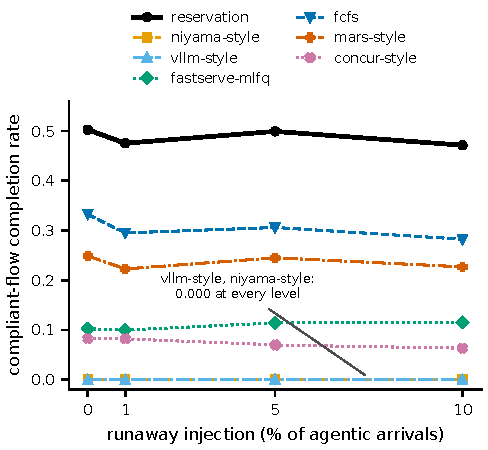
\includegraphics[width=3.25in]{figures/F4_containment_starvation.pdf}
\caption{Compliant-flow completion under adversarial runaway injection, absolute rates. The reservation discipline holds near 0.5 with a worst-case degradation of 3.1 points; FCFS completes 0.33 with no containment; the two strongest request-oriented baselines complete zero compliant flows at every level including no injection, instrumented admission starvation (one of 107 compliant flows ever scheduled, zero preemptions; Section 6.1). Deltas against zero are undefined, which is why rates are absolute.}
\label{fig:containment}
\end{figure}

This is not a missing measurement. Instrumentation of the cell shows
those policies schedule 1 of 107 compliant agentic flows, with zero
preemptions. Under interactive-class priority, long flows never receive a
device slot while interactive traffic saturates the cluster. The failure
is admission starvation rather than preemption churn, and the result is
locked by a regression test. A delta against zero is undefined, which is
why this section reports absolute completion rates throughout.

The starvation is also invisible to the audit mechanisms being specified
for agentic systems, and that consequence is worth stating separately
because it generalizes beyond scheduling. Those mechanisms are
event-based: they record what a flow did, which tools it called, what it
returned. A flow that is admitted, never scheduled, and still live at
the horizon produces no events to record, and a conformant audit trail
for such a flow is an honest and indefinitely long sequence of nothing
having happened. The failure consists of the absence of events, so
event-triggered analysis cannot surface it without a liveness test: the
record is complete, and the fault is invisible inside it.

Against that baseline, the discipline's cross-invocation budget does
what it was specified to do. Compliant-flow completion holds at 0.503,
0.475, 0.499 and 0.471 across injection levels, a worst-case degradation
of 3.1 points, and every runaway is cut off at exactly its budget. FCFS,
blind to class, completes 0.332 and degrades 5.0 points under injection:
no isolation and no containment, but no starvation either. The
discipline is the only policy in the set that is simultaneously above
0.3 absolute and below 3.5 points of adversarial degradation. Section 3
distinguished a priority from a contract as a matter of kind; this is
that distinction as a matter of record. Appendix G tabulates every
policy's rate at every injection level.

\subsection{The horizon lesson}

Investigating those zeros produced the campaign's most generalizable
finding, and it concerns measurement rather than scheduling. The
diagnostic that established the starvation as genuine also showed that
every sweep in the campaign was running a measurement horizon far shorter
than the workload's own timescale.

The median agentic flow requires roughly 711 seconds to complete with no
queueing at all, tool-time gaps plus decode service; the figure was first
measured at roughly 863 seconds on the diagnostic realization that
surfaced the problem, and the released generator derivation, which any
reader can run, gives 711. The build's default horizons ran 150 to 300
seconds, and at a 200-second window only about a quarter of agentic flows
could complete on an idle cluster. The primary metric counts completed
flows. A window shorter than the unit of value does not measure the
metric; it measures truncation.

The bias is not symmetric, and it points at completion-guaranteeing
policies specifically. A reservation pays its stranding cost during the
flow and collects its payoff at completion; a horizon that ends before
completion charges the full cost against zero payoff, the mechanism's
worst case by construction, while policies that never schedule long flows
at all are barely touched. Quantified on one core cell (Figure~\ref{fig:horizon}), the
discipline's deficit against the best baseline was 22.3 percent at a
300-second horizon and 7.8 percent at 1500 seconds, stable through 6000
seconds; at the longest horizon the discipline completed more flows in
absolute terms than its comparator while still losing on value-weighted
goodput, a real loss, but half the reported one.


\begin{figure}[tbp]
\centering
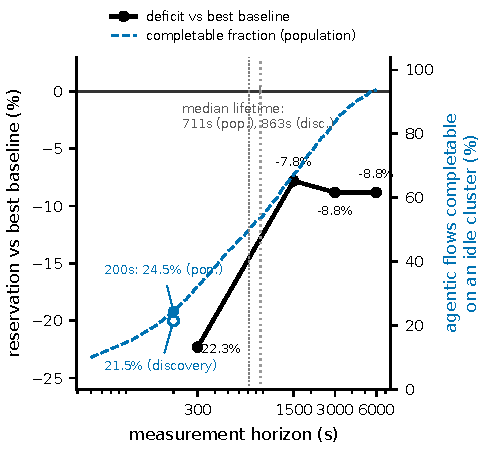
\includegraphics[width=3.25in]{figures/F5_horizon_lesson.pdf}
\caption{Horizon censoring on one core cell. The population median agentic flow lifetime, derived from the released workload generators, is roughly 711 seconds (first measured at 863 seconds on the diagnostic realization that surfaced the artifact, open markers); at a 200-second window only about a quarter of agentic flows can complete even on an idle cluster (24.5 percent of the population; 21.5 percent of the diagnostic realization), while the campaign's default horizons ran 150 to 300 seconds. The measured deficit is 22.3 percent at a 300-second horizon and halves to 7.8 percent at adequate horizons, stable through 6000 seconds. Horizons shorter than the workload's completable lifetimes charge guarantee-holders full stranding cost against zero completion payoff (Section 6.2).}
\label{fig:horizon}
\end{figure}

Censoring corrupts tuning as well as measurement. Re-tuning every policy at the corrected horizon flipped selected parameters across the board, most cleanly for the multi-level feedback baseline, whose chosen quantum moved from the shortest value in its grid to the longest in every workload family: under a censored horizon aggressive demotion looks good because long flows are truncated before their cost lands. An evaluation that had tuned at 300 seconds and measured at 1500 would have compared the mechanism against baselines mis-tuned in its favour. Both tuning campaigns are released, and the fix is structural rather than vigilant: the released code asserts before any sweep runs that the configured horizon exceeds the workload's derivable median flow lifetime, and the verdict path independently rejects any manifest whose horizon disagrees with the grid it claims to report. The correction was adopted as a numbered amendment before the final grid ran, under a one-fix clause barring further measurement changes in either direction, and its full history, including that it improved the mechanism's number on the probe cell and worsened it on the served-value comparison, is in the released amendment log. The rule generalizes to any completion-metric evaluation of long-horizon agents: horizons must exceed the completable-lifetime distribution of the workload, or the benchmark measures its own window. We found the cost of honouring it to be severe, superlinear in the horizon under sustained overload, and it forced a disclosed reduction of our own grid; we suspect the rule is widely violated for exactly that reason.

\subsection{What completion guarantees cost}

Correcting the horizon changed what the primary comparison measured, and
the corrected comparison is the verdict. Computed mechanically against
the frozen thresholds, reservation-based serving loses a median 10.3
percent of goodput per provisioned GPU-hour to the best per-cell tuned
baseline, supports the hypothesis in 0 of 108 cells against a 60 percent
requirement, and holds the interactive guardrail in 96 percent of cells.
Under the specification's thresholds, the hypothesis is killed. The
per-cell improvements are plotted in Appendix G.

The loss has structure worth more than its median. Across offered load
it is U-shaped: at 0.7x capacity the deficit runs 6.6 to 16.1 percent;
at 1.0x it is deepest, 22.4 to 23.6 percent in every cell; at 1.3x it
recovers to 9.5 to 11.5 percent; and at 1.5x the sign flips, with
reservation ahead by 0.8 to 3.2 percent in all 24 non-guardrail-failing
cells. The deficit peaks exactly where the cluster is well-provisioned:
at nominal load the work-conserving baselines run at maximum efficiency
while reservations strand capacity across idle gaps, and as load rises
past saturation the baselines begin to thrash while stranding matters
relatively less, until the ordering inverts at the top of the region.
Completion guarantees, on this evidence, are most expensive precisely
when the fleet is sized correctly.

The other axes are quieter. Cluster size is nearly flat: 8-, 16- and
32-device cells agree within roughly a point throughout, which bears on
the amendment that reduced the device axis, since nothing in the
measured trend suggests the removed 64-device axis behaves categorically
differently. Idle-gap distribution has a mild, consistent effect: longer
gap medians shrink the deficit at low load, because they favour the
tiered-pin embodiment's spill-and-restore over holding hot capacity. At
three seeds the paired bootstrap intervals are tight and solidly
negative in the load 1.0 band, wider at 0.7x where several upper bounds
cross zero. The verdict does not depend on how those intervals are read:
taking every cell at its most favourable bound, 33 of 108 would reach
the support threshold, against the 65 the criterion requires. Both the
cluster-size agreement and the per-cell intervals are read from the full
table in Appendix H.

\subsection{What they buy, and where it inverts}

The guardrail was pre-registered as a constraint, interactive p95
time-to-first-token degraded no more than 5 percent, and the mechanism
did not merely satisfy it: in most of the region it inverted it. At and
above nominal load, reservations improve interactive tail latency by
63.3 to 97.1 percent relative to the best baseline, above 90 percent in
most such cells, while reserved-idle fraction runs 93 to 100 percent in
77 of 81 such cells. Three load-1.5 cells sit at 88.9 percent, admission
having granted few reservations there, and one cell is degenerate at
zero, admission having granted none. Read together with Section 6.3,
this is the ledger's purchase side made precise: the 9.5 to 23.6 percent
goodput deficit buys near-order-of-magnitude tail-latency protection for
interactive traffic, by structurally keeping long flows off the shared
pool. Operators who price interactive tail latency highly are buying
exactly this, and today they buy it by overprovisioning; the discipline
prices the same isolation in stranded capacity instead. Both per-cell
series, tail latency and reserved-idle fraction, are plotted in Appendix
G.

The purchase fails in one measured corner. At heavy agentic mix,
overload, and short gaps, the guardrail fails spectacularly, interactive
p95 time-to-first-token worse by 468.6 to 526.5 percent across all three
cluster sizes. The mechanism is legible: with half the token volume
agentic, gaps short enough that reserved flows cycle almost
continuously, and offered load half again over capacity, the reserved
subset occupies the machine and interactive traffic starves on the
residue. Isolation is a property of the regime rather than of the
mechanism, and it reverses exactly where reservations are densest and
the machine is most oversubscribed. One further isolated failure, at low
agentic mix and nominal load against a FastServe baseline, does not
repeat at any neighbouring cell.

\subsection{Secondary hypotheses and ablations}

The second pre-registered hypothesis held that degradation keyed to
committed headroom yields a better served-value curve under overload
than deterministic demotion and preempt-and-requeue. It does not. Over
the full load sweep from 0.5x to 3.0x, the discipline's served-value
area under curve is 0.626 against the best baseline's 0.648, a 3.4
percent deficit, with two further baselines ahead of it. The comparison
carries only corrected-horizon data: an earlier censored-horizon reading
was ruled unverified and excluded from the released record, and Section
6.2 explains why censored-horizon comparisons mislead. Two baselines
collapse under overload on this metric, both of which protect the system
by throttling intake and pay for it in served value. The full sweep,
with every policy's curve and area, is in Appendix G. One
characterisation requires care. Our implementation of the
deadline-ordered family uses a demotion ladder, while the work it is
named for relegates violating requests to an opportunistic queue rather
than demoting them, so the comparison here is against the deadline
discipline rather than against that system's degradation mechanism. The
distinction does not enter the number: under the equal-budget protocol
the tuner drove that policy's demotion threshold to its maximum in every
workload family, so demotion never fires at the tuned point and the
comparison is effectively against deadline-ordered scheduling with
preemption. A second divergence is not neutralised that way: the
published scheduler interpolates between deadline order and
remaining-work order, while ours orders by class and then deadline
alone.

The ablation campaign removes one element at a time from the tuned
discipline at two operating points: an uncontended nominal-load cell, and
a contended cell with four times the decode slots, elevated load, and the
grid's shortest gaps. Across both, no element shows an effect on the
primary metric distinguishable from seed noise. At the contended cell the
total goodput spread across all nine variants is 0.68 percent against a
within-variant seed spread whose median is 29 percent. One apparent
effect appeared and did not survive: at the nominal cell, replacing
headroom-keyed degradation with queue-depth keying improved goodput by
20.9 percent, but the effect vanished at the contended cell and sits
within the nominal cell's own seed spread; an earlier internal readout
called it corroborating evidence, and that reading is withdrawn in the
released, corrected document. With three seeds a per-element median is a
draw from a distribution wider than the effects being measured, and this
design cannot separate an inert element from an unexercised one. That
noise floor is a property of the ablation design rather than of the
primary comparison: the per-cell deltas of Section 6.3 are paired, every
policy scoring byte-identical workload realizations, which cancels the
workload draw that dominates the unpaired spread here.

What the campaign does establish is robust because it is large and
consistent rather than a difference between near-identical numbers.
Reserved capacity sits 88 to 95 percent idle across both ablation
operating points, a wider and lower band than Section 6.4's because it
includes the contended cell rather than only the at-or-above-nominal
grid cells, despite the contended cell's quadrupled slots, elevated load
and minimal gaps. An agentic flow runs a short invocation and then waits
in tool time, a duty cycle of roughly 5 percent by construction, so
capacity reserved for such flows is stranded nine parts in ten
regardless of configuration. The mechanism's cost is not located in any
single element; it is located in the duty cycle of the workload the
mechanism reserves for. The tuning campaign's independent result points
the same way at larger scale: under the equal-budget protocol the tuner
drove the reserved-subset bound to its grid floor, 5 percent, in every
workload family at both horizons; the tuned-parameter table in Appendix
G shows the corrected-horizon campaign, and both campaigns are released.
Optimized truthfully, the mechanism minimizes itself.

\subsection{Fidelity: what the numbers are conditioned on}

Every number above is conditioned on the simulator's service model, so
the evaluation measured which of that model's constants the result
actually depends on rather than asserting that it does not depend on
them.

One constant binds and it is material. The single-stream decode rate
sets service time: at 0.7x the anchored value, the representative cell's
deficit compresses from 21.5 to 4.4 percent; at 1.3x it is 13.0 percent.
The sign of the verdict is robust across the tested range while the
magnitude is uncertain at roughly the factor the anchor itself is
uncertain. That is the paper's principal fidelity caveat, and it is
unresolvable here because the hardware phase was gated on this
evaluation supporting the mechanism and the gate closed. Appendix G
tabulates the per-constant figures.

Two further constants, peak decode rate and cache bytes per token, do not
move the representative cell's result at all, and the released binding
analysis shows why with instrumentation rather than assertion. At 16
decode slots the batch is capped below the size at which peak decode can
bind, and it was the binding term in 0 of 19,342 decode calls; peak
memory occupancy stays near 39 percent of capacity, so a 30 percent
perturbation changes no placement decision. The same instrumentation was
then run at a deliberately memory-bound configuration, 64 slots with an
agentic-heavy mix at elevated load, where both constants demonstrably
bind: peak decode governs 43 percent of decode calls and memory
saturates. The harness therefore detects binding where binding exists,
and the main grid's device configuration sits in the compute-bound
regime. Regression tests pin all three properties.
